\documentclass[runningheads]{llncs}
\usepackage{times}
\usepackage{amsmath}
\usepackage{amssymb}
\usepackage[noend]{algcompatible}
\usepackage[ruled,linesnumbered,noend,oldcommands]{algorithm2e}
\usepackage[T1]{fontenc}
\usepackage{hyperref}
\usepackage{xspace}
\usepackage{graphicx}
\usepackage{listings}
\usepackage{xcolor}
\lstset { %
  language=C++,
  % backgroundcolor=\color{black!5}, % set backgroundcolor
  basicstyle=\footnotesize,% basic font setting
}

\renewcommand{\note}[1]{{\color{red}{#1}}}

\title{Trail Saving on Backtrack}
\author{Randy Hickey \and Fahiem Bacchus}
\institute{Department of Computer Science, University of Toronto, Canada, 
  \email{rgh000@gmail.com, fbacchus@cs.toronto.edu}}

\begin{document}
\maketitle
\begin{abstract}
\end{abstract}

\section{Introduction}
\note{Fix later---also \cite{DBLP:journals/jsat/TakRH11} can't be
  first use of trail savings?}

The vast majority of modern SAT solvers that are used to solve
real-world problems are based on the conflict-driven clause learning
(CDCL) algorithm. In a CDCL SAT solver, backtracking occurs after
every conflict, where all literals from one or more decision levels
become unassigned, before the solver resumes making decisions and
performing unit propagations. Traditionally, CDCL solvers would
backtrack non-chronologically to the conflict level, which is the
second highest decision level remaining in the conflict clause after
conflict analysis has resolved away all but one literal from the
current decision level \cite{DBLP:conf/dac/MoskewiczMZZM01}. Recently,
however, it has been shown that backtracking chronologically
(i.e. backtracking one level only after conflict analysis)
\cite{DBLP:conf/lpar/2013,DBLP:conf/sat/NadelR18} can be effective on
many instances and was implemented in solvers that won the last two
SAT competitions. Although chronological backtracking breaks some of
the conventional invariants of CDCL solvers, it has been formalized
and proven correct \cite{DBLP:conf/sat/MohleB19}.

There are at least two possible side-effects of chronological
backtracking which may explain its effectiveness. It has been observed
that when a solver backtracks non-chronologically after a conflict,
many of the literals that are unassigned during the backtrack will be
re-assigned again in roughly the same order when the solver
continues. By using chronological backtracking, the solver keeps a lot
more of its partial assignment intact and saves from having to
reconstruct a lot of the trail via propagation that it otherwise would
have. Saving from having to reconstruct portions of the trail after
backtracking was first introduced in the context of restarts
\cite{DBLP:journals/jsat/TakRH11}. The second side-effect of
chronological backtracking is that it forces the solver to stay in the
same local neighbourhood during search, since it unassigns less of the
partial assignment and one could argue that this might lead to finding
additional conflicts more quickly or reaching a satisfying assignment
(if one exists) more quickly. However, this second side-effect also
leads to less search flexibility, since the solver does not jump out
of local neighbourhoods as often and does not obey the variable
selection heuristic. We will argue that it is the first side-effect
that leads to the effectiveness of chronological backtracking and not
the second by developing a technique which also saves from having to
repeat propagations, but allows the search to remain flexible and obey
the variable selection heuristic.

Our alternative method is "trail saving", where we cache the part of
the trail that is unassigned during a backtrack and then attempt to
restore implied parts of it as each new decision is made. Trail saving
preserves the traditional invariants of the SAT solver and its basic
version is very simple to implement. It also allows the search to
choose the order of decisions, but helps make propagation faster. We
explore the theoretical speedup that trail saving provides, develop
some enhancements to make the idea more effective, and demonstrate
experimentally that it performs similarly well as chronological
backtracking without suffering from some of the aforementioned
drawbacks.

\section{Background}
\note{elaborate backtrack after learning a clause. Also describe
  properties of the trail (a) reason valid every reason clause is made
  unit by its prefix, (b) non-contradictory, (c) non-conflicting (no
  clause is falsified), and (d) propagation complete }

We will assume the reader is familiar with SAT solving and the basics
of the CDCL algorithm \cite{DBLP:series/faia/SilvaLM09}. We will use
the notion of a trail to represent a sequence of literals
corresponding to the current partial assignment. The literals appear
on the trail in the order in which they were assigned. Associated with
every literal on the trail is a decision level. Decision level 0
represents all literals which are implied by the formula itself and
subsequent decisions start the beginning of a new decision level. When
a literal is made true by unit propagation, the literal is given its
decision level and a reason clause, where the reason clause is the
clause that was made unit by propagation in order to imply this
literal. Most modern solvers use the two-literal watch scheme to make
unit propagation more efficient, where each clause is watched by two
non-false literals. When a watcher for a clause becomes false, a
replacement is searched for in the clause. If no such replacement
exists and the other watcher is true or unassigned, then the clause is
unit. If no such replacement exists and the other watcher is also
false, then the clause is a conflict and needs to be analyzed to
produce a learnt clause.

\section{Trail Saving}
\note{
  \begin{enumerate}
  \item Use simple backtrack and save to motivate and state the
      invariant. 
  \item Introduce notation for concatenating two trails.
  \item Name and state the invariant in text (e.g. a
      defn)---concenating the cached trail with the current trail
      yields a trail that is always reason valid, but not necessarily
      non-contradictory, non-conflicting, nor propagation complete).
  \item Proof (simple) that the invariant holds for caching on
      backtrack.
  \item On backtrack at least the asserted literal and any new
      propagants at the backtrack level are added.
  \item Prove that the invariant holds (???do we need an invariant or
      simply a property of the augmented trail) for trails with extras
      inbeween.
      $T_{\mathit{old}} + T_{\mathit{newlyAdded}} +
      T_{\mathit{saved}}$ also satisfies the invariant
  \item re-acheving propagation completeness for the augmented trail
      (a) only add one level of the cached trail at a time, and do
      unit prop after (b) only add non-contradicted decision from the
      old trail. Also note that conflicts are valid and can be learnt
      from even if the augmented trail is not propagation complete. 
  \item Finally figure out a way to formalize the extra technique of
      storing on top after repeated backtracking. 
  \item Explain how freedom for the search is maintained by makeing
      decisions then consulting the trail.
  \item 
  \end{enumerate}
}

It can be observed that a SAT solver often repeats the same
propagations over and over again during execution. Although no two
descents down the trail will ever be identical because of clause
learning, the solver will often propagate many of the same literals
with the same reasons in a similar order to what it had done
previously, especially since the order of the decisions usually
remains similar. We plan to cache the part of the trail that we are
backtracking over and use it to restore some of those literals without
propagating them from scratch.

\subsection{Storing the trail cache}

The first step that is needed to use "trail saving" is to store all of
the literals which are being unassigned during a backtrack, along with
their respective reason clauses, in a "trail cache". Decisions should
be marked with a null reason. The literals should appear in the same
order on the trail cache as they had appeared on the trail. We will
keep a pointer, which we will refer to as the "top" of the trail
cache, and initially set it to be the literal which had appeared the
earliest on the trail. Note that initially the top of the trail cache
always has a null reason (i.e., it was the start of a new decision
level on the previous trail). As the literals from the trail cache get
restored (i.e., assigned), the top of the trail cache will be updated
to the next literal not yet restored.

\begin{figure}\center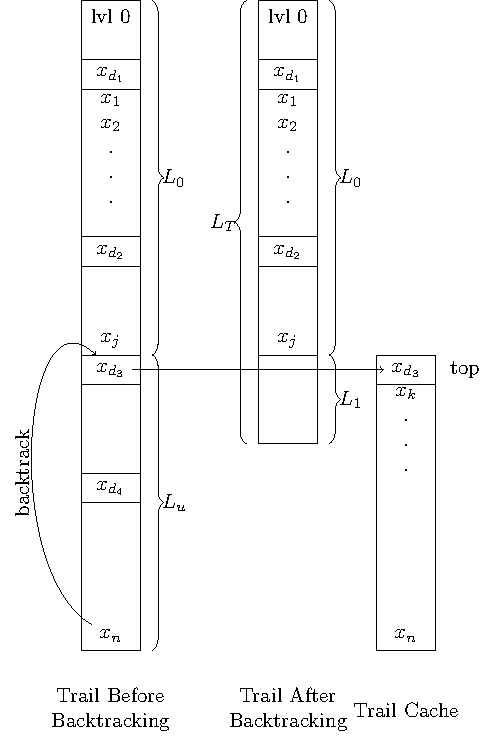
\includegraphics[scale=0.7]{figures/trail_diagram.pdf}\caption{Storing into a trail cache after backtracking.}\end{figure}

\subsection{Restoring the trail cache}
We will base trail saving on the following critical invariant. If the
top of the trail cache becomes true at any point, even after an
arbitrary number of decisions and propagations have been made since
the last backtrack, the set of literals on the trail cache after the
top and up to but excluding the next literal with a null reason is
still implied by the current trail. The top of the trail cache can
become true either by decision or unit propagation, and this invariant
still holds.\newline

\textit{Proof 1} We will refer to the set of literals that become
unassigned during the backtrack after conflict analysis has taken
place as $L_u$, and will refer to the rest of the trail that remains
assigned as $L_0$. We will refer to all of the literals that get
placed on the trail after $L_0$ during subsequent propagations and
decisions as $L_1$. We will refer to the current trail $L_0 \cup L_1$
as $L_T$. The trail cache will contain the literals in $L_u$ ordered
by their appearance on the old trail. Let $L_c[i]$ denote the set of
the first i literals on the trail cache. Let $L_c[top]$ be the top of
the old trail, which gets updated as parts of the trail cache get
restored.

The $i$th literal on the trail cache is implied by
$L_0 \cup L_c[i-1]$, as long as the $i$th literal has a non-null
reason, since $L_0 \cup L_c[i-1]$ had forced $L_c[i]$ on the previous
trail. $L_0 \subseteq L_T$, since $L_T = L_0 \cup L_1$. Therefore, the
$i$th literal on the trail cache is also implied by
$L_T \cup L_c[i-1]$.

Assume $L_c[top]$ is true, which means that
$L_c[0], ..., L_C[top] \subseteq L_1 \subseteq L_T$. Then, from above,
every literal on the trail cache up to but excluding the next literal
with a nun-null reason would be implied. $\blacksquare$\newline

Once the backtrack has been completed and the solver resumes with
decisions and propagations, we will attempt to restore parts of the
trail cache automatically during propagation to make it faster by
using the invariant stated above. Each time the propagation routine is
about to propagate a new literal, we first check the top of the trail
cache to determine its truth value. If that literal's truth value is
already true, we assign all of the literals that come after it on the
trail cache to be true up until (and excluding) the next literal with
a null reason.

A potentially quadratic speedup can be realized during the propagation
of these literals since they are being propagated as a set, rather
than one at a time, as argued in \cite{DBLP:conf/sat/HickeyB19,DBLP:journals/jair/Gent13}. Restoring literals from the trail cache
automatically not only leads to quicker propagation of future
literals, but also means that the propagation routine has less work to
do as it searches for new watchers in clauses on watchlists. All of
the reasons attached to these literals that are automatically restored
will now be satisfied, thus the propagation routine can skip over them
rather than having to access each of them potentially multiple times
to find they are unit.

If at any time the top of the trail cache is a literal $l$ with a
non-null reason whose truth value is already false, we determine a
conflict has occurred with the conflict clause being $l$'s reason from
the trail cache. This is because we know from Proof 1 that $l$ is
implied to be true at this point by the reason on the trail cache
(i.e., the reason on the trail cache is unit), but $\lnot l$ was also
previously assigned to be true, therefore we have a conflict. This
leads to a third potential speed up, since a conflict has been
detected and none of the pending propagations have to be
completed. Since trail saving can sometimes save hundreds or thousands
of literals at a time, the number of propagations required to detect a
conflict could be very costly.

\begin{algorithm}
  	\TitleOfAlgo{propagate()}
	\begin{algorithmic}[1]
        \WHILE{queue not empty}
        \STATE { }
        \STATE restoreTrailCache()
        \STATE { }
        \STATE $l := $ next literal on queue
        \FOR{each clause $c \in $ watchlist($\neg l$)}
		\FOR{each literal $x \in c$}
        \IF{$val($x$) \neq$ false and x is not already a watcher of c}
        \STATE let $x$ be a watcher of $c$ and add $c$ to watchlist($\neg x$)
        \STATE break
        \ENDIF
		\ENDFOR
		\IF{no new watcher was found}
        \IF{other watcher $x_2$ of $c = $ false}
        \STATE return c as conflict
        \ELSIF{other watcher $x_2$ of $c$ is unassigned}
        \STATE enqueue $x_2$
        \ENDIF
		\ENDIF
        \ENDFOR
        \ENDWHILE
	\end{algorithmic}
\end{algorithm}

\begin{algorithm}
  	\TitleOfAlgo{restoreTrailCache()}
	\begin{algorithmic}[1]
        \IF{trail saving turned on}
		\STATE{let tc $=$ top of trail cache}
		\IF{val(top of trail cache) $=$ true}
        \WHILE{trail cache not empty}
        \STATE{move top of trail cache (tc) to next literal}
        \IF{reason(tc) is null}
        \STATE{break}
        \ELSIF{val(tc) $=$ false}
        \STATE{return conflict with reason(tc)}
        \ELSIF{val(tc) $=$ unassigned}
        \STATE{enqueue tc with reason reason(tc)}
        \ENDIF
        \ENDWHILE
		\ENDIF
        \ENDIF
	\end{algorithmic}
\end{algorithm}

\subsection{Enhancements}

In the standard version of trail saving outlined above, the trail
cache needs to be deleted after each backtrack in order to make room
for the new backtracked literals to be cached. The first enhancement
to trail saving is to keep the trail cache intact instead of clearing
it before each backtrack, and to add the literals that will be
backtracked over to the beginning of the already existing trail
cache. In order to preserve soundness, we must add the literals from
the current backtrack to the beginning of the trail cache, such that
the trail cache has as its prefix the literals which are being
backtracked over, and as its suffix the previous trail cache. \newline

\textit{Proof 2} We will use all of the same set names as Proof 1 and
also refer to the set of literals on our previous trail cache as
$L_{pc}$. We concatenate the literals in $L_{pc}$ to the end of $L_c$
to get $L_{sc}$. We know that $L_{pc}$ is a valid trail cache for
$L_0 \cup L_u$. If we reach the end of $L_c$ without any conflicts, we
know that $L_u \subseteq L_T$. Since $L_0 \subseteq L_T$, then
$L_u \cup L_0 \subseteq L_T$ and therefore $L_{pc}$ is a valid trail
cache for $L_T$. $\blacksquare$\newline

In order for the previous trail cache to be of any use, one must
actually never store the last level of the current trail to the trail
cache at all, since a learnt clause prevents the last level from being
duplicated in the future. If any part of the previous trail cache was
used to construct this last level, it must also be discarded from the
previous trail cache before the previous trail cache is concatenated
to the end.

When concatenating trail caches together as above, it is important to
note that the running trail cache can grow indefinitely. The trail
cache can be trimmed periodically in the following way. Traverse down
the trail cache and whenever a literal appears more than once, delete
its entry in the trail cache. Whenever a literal $x$ appears whose
complement $\lnot x$ has already appeared on the trail cache, $x$
should be deleted and everything remaining until the end of the trail
cache should be deleted (in order to keep the trail cache free of
conflicts).  We decided to trim the trail cache whenever its size
exceeded twice the total number of variables in the SAT instance, as
that is what worked best in preliminary experiments.\newline

The next enhancement to trail saving is to scan the trail cache to
check if there is a literal that is already assigned false within some
limit. The limit we found worked best is to scan the trail until the
third null reason is found (i.e. "looking ahead 2 decisions"). If a
literal that is already assigned false is found, we know that we are
guaranteed to have a conflict in the near future, and we force the SAT
solver's subsequent decisions to come from the trail cache instead of
using the regular variable selection heuristic.

Sometimes using trail saving to automatically restore literals with
their previous reasons will lead to a literal getting a reason that is
"worse" (in terms of number of literals, but one could use a different
metric) than the reason it would have ended up with under normal
propagation (i.e. without trail saving). The last enhancement we made
to trail saving was to stop restoring literals from the old trail as
soon as we hit a reason that we suspected might be "bad". For this, we
kept a running mean and standard deviation of the length of all
reasons used in the solver so far, and decided to stop restoring from
the trail whenever we hit a reason that was greater in length than two
standard deviations above the mean length. This way, when normal
propagation resumes, we give it a chance to find a better reason than
the one that trail saving had stored from the last descent down the
trail.

Another potential enhancement one could use is to use the trail cache
to try to learn a second clause automatically when the solver reaches
a conflict. However, we did not find a way to implement this to make
it beneficial and the number of levels we have to scan for a second
conflict would have to be more than the number of levels we already
look ahead on each decision (when the solver is not under conflict).

\section{Related Work}
\subsection{Trail Saving for Assumption-Based SAT}
Trail saving was briefly introduced in the context of assumption-based
SAT \cite{DBLP:conf/sat/HickeyB19} in order to speed up the
propagation of the assumptions each time the solver backtracked past
the assumption levels. Note that the process is the same, but it only
works to restore the propagants and implicants of the assumptions and
only after a learnt unit clause. Becuase the number of propagants and
implicants of the assumptions tends to become dominated by the number
of assumptions in the applications it was tested on, the technique did
not yield a significant improvement. It would be interesting to
combine the extended version of trail saving outlined in this paper
with trail saving over the assumptions to see if that could produce
better results.

\subsection{Comparison to Chronological Backtracking}
As mentioned earlier, chronological backtracking also achieves some of
the theoretical speedups that trail saving achieves. One advantage of
chronological backtracking is that it does not require any caching of
the trail or accessing such a cache during propagation; it simply
leaves a vast portion of the trail intact rather than backtracking all
the way to the conflict level. Chronological backtracking will also
speed up propagations slightly more than trail saving, because it
leaves more literals assigned at once which leads to clauses being
detected as unit more quickly.

One disadvantage that chronological backtracking has compared to trail
saving is that it doesn't allow the search as much flexibility to jump
out of local neighbourhoods, as the common variable selection
heuristics tend to depend on
\cite{DBLP:conf/dac/MoskewiczMZZM01,DBLP:conf/sat/2015,DBLP:conf/sat/LiangGPC16}. Because
chronological backtracking leaves a large portion of the trail
assigned, it will behave similarly to how the solver would behave if
it was to force the decisions that do occur within this large portion
of literals, whereas trail saving does not force any decisions. As
variable selection heuristics become more refined, it is likely that
adhering to them will become more crucial to performance.

Another disadvantage is that, because propagation is not performed at
every decision level, literals that remain assigned during
chronological backtracking (but otherwise would have been unassigned)
do not have a chance to move their decision levels up. An example of
this is when the solver was supposed to backtrack over a literal that
would end up being unit propagated at level 0, but stays assigned at
its current decision level when chronological backtracking is
used. This could potentially effect the lbd score or length of the
learnt clause that gets generated at the next conflict. Additionally,
chronological backtracking breaks the invarant that all literals
appear on the trail in monotonically increasing order by decision
level, which makes its implementation slightly more complicated.

\section{Experiments and Results}
For the version of cadical published in
\cite{DBLP:conf/sat/MohleB19}chronological backtracking gives solves 6
more problems and has a lower Par-2 score by a decent margin. When
adding trail saving and all enhancements to the default
non-chronological version of cadical, we end up solving 4 more problems
and the Par-2 score goes decreases by a margin not as good as that
produced by the non-chronological backtracking version. The trail saving
versions improve on the standard non-chronological backtracking but do
slightly worse than the chronological backtracking versions.

For the latest version of cadical that we downloaded as of January 1,
2020, chronological backtracking (set to default parameters)
interestingly makes the solver perform worse than standard
non-chronological backtracking does. This shows that not all solvers
will benefit from chronological backtracking; it depends on the solver's
mix of heuristics and may require fine-tuning the parameters associated
with chronological backtracking. However, after implementing trail
saving and enhancements on top of this version of cadical with
non-chronological backtracking, the solver performs roughly the same as
it does with standard non-chronological backtracking, and does not
suffer a slow down as chronological backtracking appears to.

For MapleSat, chronological backtracking makes a significant improvement
on MapleLCMDist both in terms of total number of problems solved and
Par-2 score. Similarly, trail saving implemented on top of MapleLCMDist
with non-chronological backtracking receives a similarly significant
improvement in terms of total instances solved and Par-2 score, and
actually outperforms chronological backtracking on both measures.

\begin{figure}
    \begin{tabular}{|l|l|l|l|l|l|}
      \hline
      & Total Solved & SAT & UNSAT & Par-2 (x 10\textasciicircum{}6 s) \\ \hline
      cadical                  & 532          & 314 &  218  & 3.220                             \\ \hline
      cadical\_chrono          & 525          & 308 &  217  & 3.269                             \\ \hline
      cadical\_trail           & 529          & 310 &  219  & 3.248                             \\ \hline
      cadical\_trail\_enhanced & 531          & 313 &  218  & 3.216                             \\ \hline
    \end{tabular}
    \caption{Table of results for cadical, version pulled from github as of January 1, 2020.}
\end{figure}

\begin{figure}
    \begin{tabular}{|l|l|l|l|l|l|}
      \hline
      & Total Solved & SAT & UNSAT & Par-2 (x 10\textasciicircum{}6 s) \\ \hline
      cadical                  & 492          & 289 &  203  & 3.5020                            \\ \hline
      cadical\_chrono          & 498          & 292 &  206  & 3.4400                            \\ \hline
      cadical\_trail           & 493          & 290 &  203  & 3.5228                            \\ \hline
      cadical\_trail\_enhanced & 496          & 292 &  204  & 3.4847                            \\ \hline
    \end{tabular}
    \caption{Table of results for cadical or "chrono", version published in \cite{DBLP:conf/sat/MohleB19}.}
\end{figure}

\begin{figure}
    \begin{tabular}{|l|l|l|l|l|l|}
      \hline
      & Total Solved & SAT & UNSAT & Par-2 (x 10\textasciicircum{}6 s) \\ \hline
      maple           & 458          & 259 &  199  & 3.797                             \\ \hline
      maple\_chrono   & 470          & 271 &  199  & 3.690                             \\ \hline
      maple\_trail    & 472          & 271 &  201  & 3.694                             \\ \hline
      maple\_enhanced & 473          & 277 &  195  & 3.667                             \\ \hline
    \end{tabular}
    \caption{Table of results for MapleLCMDist.}
\end{figure}
\clearpage

\section{Future Work}

With more clever data structures the efficiency of restoring the trail
could be improved. There are a number of parameters which can be
tuned, including how often to refresh the trail, how large the cutoff
point for rejecting "long" reasons should be, how long to wait to
prune the trail cache if one is appending multiple trail caches
together, how far to look ahead on the trail cache for conflicts (in
terms of number of decisions or total number of literals). We only
experimented with a few different settings of these parameters that
made sense, but more careful fine-tuning of these parameters could
further enhance the effectiveness of the technique. There are
potentially other techniques one could use a trail cache for,
including inprocessing steps that involve probing. A look down the
trail cache is an incomplete but very fast way to do a probing step,
as opposed to propagation. It is also possible that trail saving and
chronological backtracking could be combined in some way to produce
even better results.

\bibliography{sat}{}
\bibliographystyle{splncs04}
\end{document}

\iffalse \textit{Example 1} Suppose the literal $y$ can be restored
from the trail cache, and its reason clause $cr$ contains the literals
${y \lnot x_1, \lnot x_2, ..., \lnot x_n}$. This means that
$x1, ..., x_n$ have become true and are currently on the
trail. Suppose $x_n$ is the most recent literal on the trail and
Without trail saving, the propagation routine will have to access $cr$
from the watchlist of one of the literals $\blacksquare$\newline

\textit{Example 1} Suppose the literals $x_1, ... x_n$ are on the
trail cache, with none of them having a null reason, and $x_1$ becomes
true (e.g., the solver makes a decision for $x_1$ to be true). Then,
$x_2, ... x_n$ are implied by the current trail. Now we will examine
the propagation of a clause c which consists of the literals
$l, \lnot x_1, \lnot x_2, ..., \lnot x_n$ with and without trail
saving. Assume $l$ and $\lnot x_1$ are the current watched literals.

Without trail saving, $\lnot x_1$ becomes false and a new watcher is
searched for and found 1 literal later, $\lnot x_2$, and then
$\lnot x_1$ and $\lnot x_2$ are swapped. Next $\lnot x_2$ becomes
false, a new watcher is searched for and found 2 literals later,
$\lnot x_3$, and then $\lnot x_2$ and $\lnot x_3$ are swapped. This
process will continue until all $x_n$ literals are false, c becomes
unit, and $l$ becomes forced to be true. This propagation took
$1 + 2 + ... + n$ searches through clause c, for a total of $O(n^2)$
searches.

With trail saving, $x2, ... x_n$ are all assigned to be true as soon
as $x_1$ is made true, so immediately the values of literals
$\lnot x_1, ..., \lnot x_n$ in c are false. During propagation, a new
watcher is searched for to replace $\lnot x_2$, n literals are
saerched over without finding any, thus c is detected as unit and $l$
becomes forced to be true. This propagation took $O(n)$ searches
through clause c. $\blacksquare$\newline \fi

\iffalse
\begin{figure}\includegraphics[scale=0.8]{figures/cactus_cadical.pdf}\caption{\small{Comparison
        of run times for versions of cadical. cadical is without
        chronological backtracking, cadical-chrono is with
        chronological backtracking, cadical-trail is with the first
        version of trail saving, cadical-trail-2levels-ahead is the
        trail saving with all enhancements added.}}\end{figure}
\begin{figure}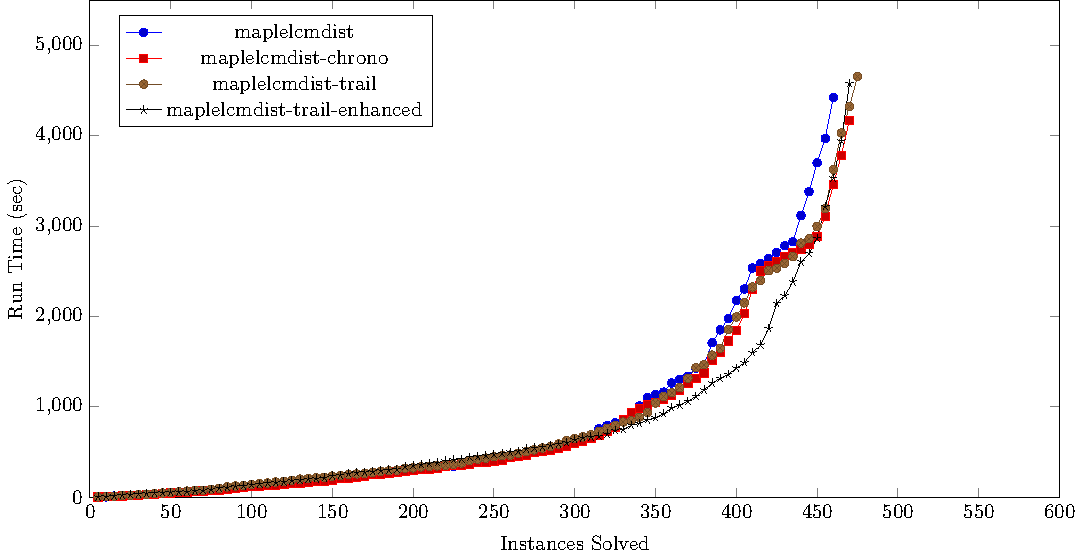
\includegraphics[scale=0.8]{figures/cactus_maple2.pdf}\caption{\small{Comparison
        of run times for versions of MapleSAT. maplelcmdist is from
        the 2017 SAT Competition, maplelecmdist-chrono is with
        chronological backtracking (2018 SAT Competition),
        maplelcmdist-trail is with the first version of trail saving,
        maplelcmdist-trail-enhanced is with trail saving and all
        enhancements added.}}\end{figure}
\begin{figure}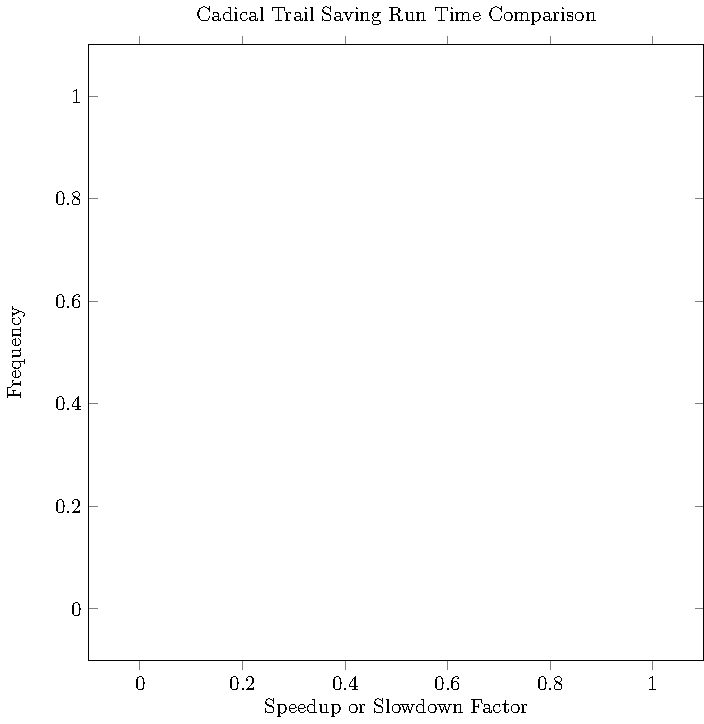
\includegraphics[scale=0.8]{figures/test.pdf}\caption{}\end{figure}
\begin{figure}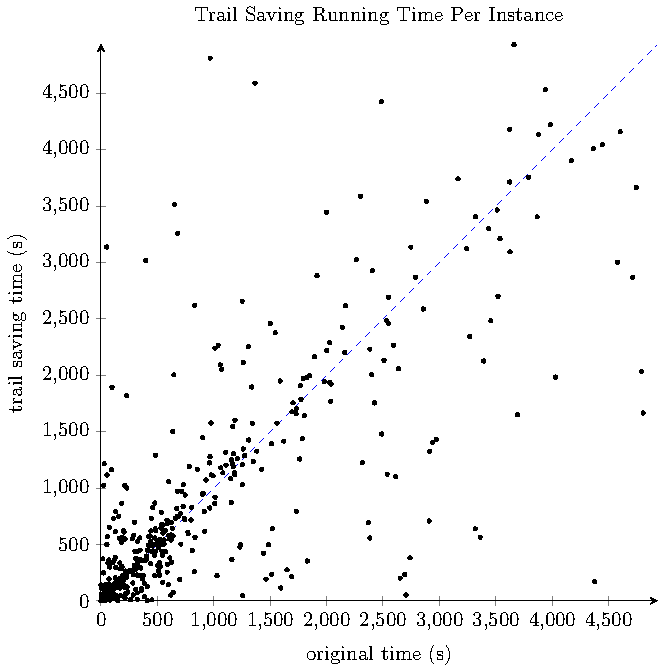
\includegraphics[scale=0.8]{figures/test2.pdf}\caption{}\end{figure}
\fi
\iffalse
\begin{figure}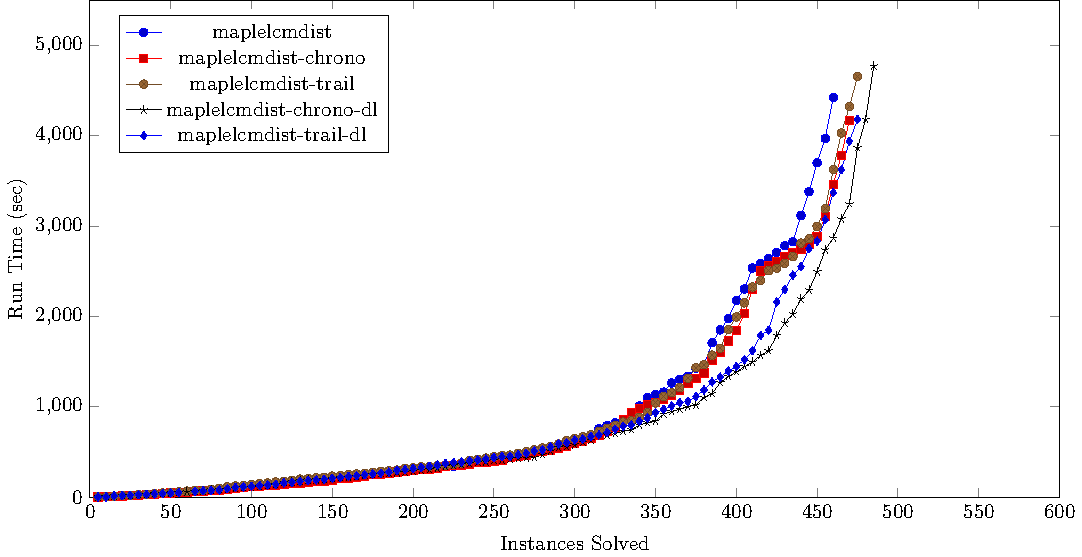
\includegraphics[scale=0.8]{figures/cactus_maple.pdf}\caption{\small{Comparison
        of run times for versions of MapleSAT. maplelcmdist is from
        the 2017 SAT Competition, maplelecmdist-chrono is with
        chronological backtracking (2018 SAT Competition),
        maplelcmdist-trail is with the first version of trail saving,
        maplelcmdist-chrono-dl is with chronological backtracking and
        duplicate learnts (2019 SAT Competition),
        maplelcmdist-trail-dl is with trail saving and duplicate
        learnts}}\end{figure}
\fi

\iffalse
\begin{figure}[t]
    \begin{center}
        \fss{9pt}{10pt}
        \setlength\tabcolsep{1pt}
        \begin{tabular}{| p{4.2cm} | c | c | c | c | c | c | c | c |}
          \hline
          & \multicolumn{4}{|c|}{Total} & \multicolumn{2}{|c|}{Unweighted} & \multicolumn{2}{|c|}{Weighted} \\ \hline
          & MaxHS & +/- & \hspace{1pt} RC2 \hspace{1pt} & +/- & MaxHS & \hspace{1pt} RC2 \hspace{1pt} & MaxHS & \hspace{1pt} RC2 \hspace{1pt} \\ \hline
          original & 6052 & 0/0 & 6030 & 0/0 & 3940 & 3993 & 2112 & 2037 \\ \hline
          enqueue assumptions as set & 6131 & 114/35 & 6081 & \hspace{0.5pt} 99/48 \hspace{0.5pt} & 3995 & 4032 & 2136 & 2049 \\ \hline
          enqueue assumptions as set + \newline save literals after learnt units & 6136 & 120/36 & 6079 & \hspace{0.5pt} 95/46 \hspace{0.5pt} & 3991 & 4030 & 2145 & 2049 \\ \hline
          enqueue assumptions as set + \newline save literals after learnt units + \newline save literals from last invocation & 6138 & 115/29 & 6080 & \hspace{0.5pt} 92/42 \hspace{0.5pt} & 3989 & 4030 & 2149 & 2050 \\ \hline
        \end{tabular}
    \end{center}
    \caption{Number of \maxsat instances solved by MaxHS and RC2 using
      different extensions of the underlying \sat solver. The +/- column shows
      the number of instances gained/lost vs the original.}
    \label{fig:nsolved}
\end{figure}
\fi
